\chapter{Modelagem de Ameaças} \label{cap:modelagemameacas}

\section{Escopo, ativos e objetivos de segurança}


O objetivo deste capítulo é modelar a implementação de uma comunicação com autenticidade entre\textit{dongle} e um servidor externo, tendo como intermediário um \textit{app mobile} que se comunica com o \textit{dongle} por meio de \textit{BLE} e não pode ser confiado. Os dados devem trafegar para o servidor de modo que, ao recebê-los, deve ser criptograficamente garantido que eles foram medidos a partir do dongle que se identifica como originador do dado, a fim de que não seja possível alterar o conteúdo das medições ou deliberadamente esconder informação entre duas mediçõesdiferentes sem que o servidor consiga detectar.

O objetivo principal para o contexto deste trabalho é que as informações medidas pelo dongle que chegam no servidor possam ser confiadas e usadas para análises seguras a respeito do funcionamento do carro e como ele está sendo conduzido. Assim, deve-se garantir autenticidade ou seja, todo registro recebido pelo servidor deve ter sido gerado pelo dongle associado a ele integridade, ou seja, o dado que é recebido pelo servidor não pode ter sido alterado; unicidade, ou seja, os registros devem ser recebidos uma única vez e a ordem em que eles foram gerados dev ser mantida; e completude detectável, ou seja, o servidor deve saber exatamente se e quais registro estão faltando ao sincronizar com o \textit{dongle}.

%e vínculo ao veículo, o que garante que o servidor consegue identificar quando há troca de veículo entre os \textit{boots} do dongle.

\section{Fronteiras de Confiança}

Nesse contexto, só é possível confiar plenamente no dongle e no servidor. Assim, o app e os enlaces BLE e internet são modelados como não confiáveis, conforme a \autoref{fig:fronteiras-confianca}.

\begin{figure}[H]
	\centering
	\caption{Fronteiras de confiança entre \textit{dongle}, \textit{app} e servidor}
	\label{fig:fronteiras-confianca}
	% Fonte PlantUML: ../assets/aux-docs/plantuml/fronteiras-confianca.puml
	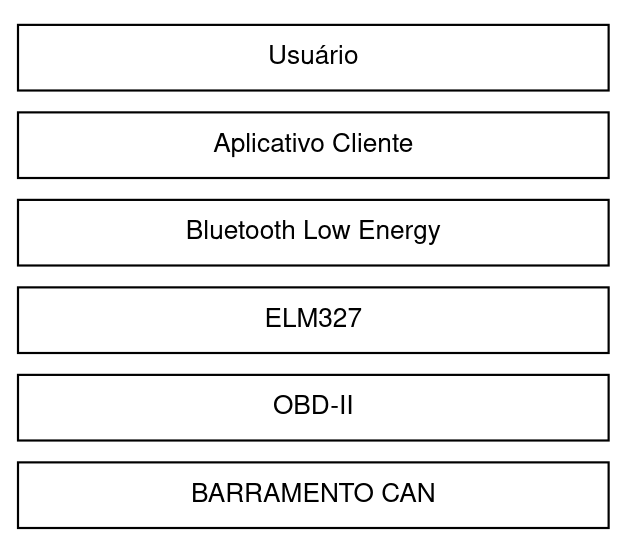
\includegraphics[width=\textwidth]{assets/cap2-conceitos/camadas.png}
	\legend{Fonte: elaborado pelo autor.}
\end{figure}

\section{Adversários}

Existem diversos adversários e ataques que podem ser modelados no cenário, envolvendo os diferentes componentes e ligações entre eles. É possível dividir os ataques em três principais categorias. Dentro das categorias de ataque, também é possível definir cinco tipos principais de adversários que aparecem entre elas:

\begin{itemize}
    \item (AD1) o terceiro perto do carro que pode ter acesso ao enlace de rádio do BLE, cujo objetivo é espionar ou injetar dados;
    \item (AD2) o próprio motorista que tem acesso ao app original do sistema, cujo objetivo é esconder, alterar medidas do dongle ou enviar as medidas do dongle para terceiros não autorizados;
    \item (AD3) um app de terceiro no celular pareado que pode acessar as características BLE, cujo objetivo é coletar as informações medidas para outros propósitos;
    \item (AD4) um atacante na rede entre o celular e o servidor, cujo objetivo é ler ou alterar dados no caminho para o servidor;
    \item (AD5) um invasor no servidor que tem acesso ao banco de dados e tudo que está armazenado, cujo objetivo pode ser apagar ou forjar dados.
\end{itemize}


Para especificar os ataques, será utilizada uma metodologia de modelagem que define o adversário, a pré-condição do ataque, o método a partir do qual o ataque é executado, a vulnerabilidade que ele explora, o alvo que está sendo atacado, e, por fim, o efeito que o ataque causa.

\section{Catálogo de Ataques, por Categoria}

\subsection{Comunicação Wireless} \label{sec:comunicacao-wireless}

Esses são ataques que se concentram tanto no enlace BLE entre o app e dongle quanto na conexão de rede entre o app e o server.  Dentre eles, estão sniffing, replay, Man In The Middle (MITM), acesso direto ao dongle por um terceiro e negação de serviço do enlace. Abaixo estão modelados os ataques do ponto de vista do BLE, mas os mesmos princípios podem ser pensados para um adversário do tipo AD4 que interfere na comunicação entre o app e o servidor.

Um exemplo de ataque dessa categoria é o sniffing (A1.1), no qual o adversário do tipo AD1 pode querer obter os dados do motorista, afetando sua privacidade. A pré-condição é ter um sniffer ao alcance do sinal do BLE, cujo enlace não é cifrado. O método a partir do qual ele é feito é seguir a conexão e recuperar tudo que passa pelas características do dongle de maneira passiva. A vulnerabilidade explorada é a falta de cifração nas características BLE, o alvo são os dados transferidos pelo enlace, e o efeito é o vazamento de dados medidos pelo dongle. 

No ataque de \textit{replay} (A1.2), o adversário do tipo AD1 quer repetir comandos ou respostas para alterar o estado do dongle ou enganar o app. A pré-condição é ter capturado o tráfego por \textit{sniffing} e conseguir se conectar ao dongle ou se passar por ele. O método consiste em reescrever na característica de recepção quadros gravados anteriormente, como \texttt{AT\#DIAG 1}, \texttt{AT\#PID} ou \texttt{ATZ}, ou em se anunciar como o dongle e devolver respostas antigas ao app. A vulnerabilidade explorada é a ausência de autenticação da conexão e de garantia de frescor das mensagens, somada ao fato de o app não verificar a identidade do dongle. O alvo são o modo e a configuração do dongle e os dados exibidos pelo app, e o efeito é uma coleta pausada ou reconfigurada sem o conhecimento do motorista, ou um painel com valores falsos.

Já no \textit{Man In The Middle} (A1.3), o adversário do tipo AD1 quer ler e alterar em tempo real o que app e dongle trocam. A pré-condição é estar presente quando o app se conecta ou durante o pareamento, com dois rádios BLE. O método é conectar-se ao dongle, anunciar um clone dele ao app e repassar todo o tráfego entre os dois, alterando valores ou inserindo comandos no caminho. A vulnerabilidade explorada é que nenhum dos lados autentica o outro no enlace, o alvo é a integridade de comandos e respostas, incluindo as requisições ao barramento CAN no modo diagnóstico, e o efeito é um painel adulterado e requisições injetadas no carro.

Por fim, no acesso direto (A1.4), o adversário do tipo AD1 quer usar o dongle como se fosse o app. A pré-condição é que o dongle aceite conexões de qualquer dispositivo, e o método é simplesmente conectar-se e escrever comandos na característica de recepção, inclusive requisições ao barramento CAN no modo diagnóstico. A vulnerabilidade explorada é a falta de autenticação da conexão, agravada pelo dongle aceitar uma segunda conexão simultânea. O alvo são os dados medidos, o modo diagnóstico e a configuração do dongle, e o efeito é a leitura dos dados, a pausa da coleta e consultas ao veículo feitas em nome do dono.

Na negação de serviço do enlace (A1.5), o adversário do tipo AD1 quer impedir que o app se comunique com o dongle, atacando a
disponibilidade da conexão. A pré-condição é estar ao alcance do sinal BLE do dongle. O método é conectar-se ao dongle assim que ele começa a se anunciar e manter a conexão aberta, ocupando as conexões que ele aceita, de modo que o app oficial não consiga se conectar. A vulnerabilidade explorada é que o dongle aceita conexões de qualquer dispositivo e tem um número limitado delas. O alvo é a disponibilidade  do enlace BLE e, por consequência, a sincronização dos registros com o servidor, e o efeito é um dongle inacessível ao app: o painel deixa de ser atualizado e o servidor recebe um intervalo sem dados que não é causado pelo motorista.


\subsection{Comunicação entre Carro e Dongle} \label{sec:comunicacao-carro-dongle}

Já esses ataques acontecem no barramento CAN entre o carro e o dongle, ou seja, o atacante pode usar algum elemento externo para simular a CAN do veículo por inteiro ou para sobrescrever um determinado PID a fim de manipular leituras.

No ataque de ECU emulada (A2.1), o adversário do tipo AD2 quer que a seguradora receba uma condução melhor do que a real. A pré-condição é ter acesso físico à porta OBD e um emulador ou \textit{gateway} CAN, sendo que o próprio ECUSim deste projeto serve como prova de conceito. O método é ligar o dongle no emulador, ou colocar um \textit{gateway} entre a porta e o dongle que repassa as requisições ao carro e altera apenas as respostas escolhidas, como limitar a velocidade reportada. A vulnerabilidade explorada é que as respostas OBD-II não são autenticadas, de modo que o dongle confia em quem responder. O alvo é a veracidade dos dados medidos antes de serem assinados, e o efeito são registros autênticos com conteúdo falso: a assinatura prova que o dongle mediu, mas não que o carro disse aquilo.

Na resposta concorrente no barramento (A2.2), o adversário do tipo AD2 quer sobrescrever apenas alguns PIDs sem retirar o carro do barramento. A pré-condição é ter um dispositivo ligado ao CAN capaz de responder mais rápido que a ECU. O método é escutar as requisições funcionais, enviadas para o identificador 0x7DF, e responder em 0x7E8 antes da ECU real. A vulnerabilidade explorada é a mesma do ataque anterior, somada ao fato de o dongle aceitar a primeira resposta da faixa 0x7E8--0x7EF sem endereçar ECUs específicas. O alvo é a veracidade dos PIDs escolhidos, e o efeito, além dos registros autênticos com conteúdo falso, é um painel e um diagnóstico enganados.


\subsection{Aplicativo Malicioso}  \label{sec:app-malicioso}


Como o aplicativo será instalado no aparelho do usuário do dongle, um aparelho com \textit{root} tem total controle do funcionamento do app e pode manipulá-lo para gerar ataques ao sistema. Esses ataques podem manipular o processo de envio dos dados entre o app e o servidor a fim de fazer com que as informações do servidor não correspondam com o que foi realmente medido pelo dongle no carro. O principal adversário nesse contexto é o do tipo AD2, que controla o app e pode querer forjar cenários de medição que vão de encontro aos interesses da entidade no servidor externo, como uma seguradora ou gerenciadora de frotas. 

Na exfiltração (A3.1), o adversário do tipo AD3, ou um SDK de terceiros embutido no próprio app, quer vender ou usar para outros fins os dados de condução e de posição do motorista. A pré-condição é ter permissão de Bluetooth e de internet no celular pareado com o dongle. O método é conectar-se ao dongle quando o app oficial não está conectado e ler os dados medidos, ou ler os registros e posições que passam pelo app, enviando tudo a outro servidor. A vulnerabilidade explorada é que os dados não são cifrados na camada de aplicação e que a autorização é feita por aparelho, e não por app. O alvo é a privacidade do motorista, e o efeito é o vazamento de dados pessoais e o rastreamento do veículo.

Já na omissão de mensagens do servidor (A3.2), o adversário do tipo AD2, por meio de um app modificado, quer degradar a coleta sem que a culpa recaia sobre o app. A pré-condição é que o app seja o único caminho entre o servidor e o dongle. O método é receber do servidor o desafio, a confirmação de recebimento ou o \textit{token} de diagnóstico e não repassá-los ao dongle, ou repassar apenas alguns. A vulnerabilidade explorada é que as mensagens do servidor não têm confirmação de entrega ao dongle. O alvo é a recuperabilidade dos registros, a âncora de tempo e a troca de época, e o efeito é que, sem confirmações, a memória do dongle enche e ele descarta registros antigos; sem desafio, não há âncora de tempo nem época nova; e, sem \textit{token}, o diagnóstico é negado.

Na alteração de medições (A3.3), o adversário do tipo AD2 quer melhorar o próprio histórico. A pré-condição é controlar o app, ou um \textit{proxy} com uma autoridade certificadora instalada no celular, e o método é modificar bytes de um bloco antes de enviá-lo ao servidor. A vulnerabilidade explorada é a ausência de integridade fim a fim, o alvo é a integridade dos registros, e o efeito é a aceitação de dados falsos.

Na repetição de medições (A3.4), o adversário do tipo AD2 quer repetir uma viagem tranquila. A pré-condição é ter gravado blocos antigos, e o método é reenviar ao servidor blocos já aceitos. A vulnerabilidade explorada é a falta de garantia de unicidade, o alvo é a unicidade dos registros, e o efeito são dados duplicados no servidor. 

Na reordenação das medidas enviadas (A3.5), o adversário do tipo AD2 quer deslocar eventos no tempo. A pré-condição é controlar o app, e o método é enviar os blocos fora de ordem. A vulnerabilidade explorada é que a ordem dos registros não é garantida, o alvo é a ordem dos registros, e o efeito é uma linha do tempo falsa.

No descarte de medições intermediárias (A3.6), o adversário do tipo AD2 quer apagar um evento específico, como uma frenagem brusca. A pré-condição é controlar o app, e o método é deixar de enviar os blocos escolhidos. A vulnerabilidade explorada é a falta de completude, o alvo é a completude dos registros, e o efeito é uma lacuna silenciosa nos dados do servidor.

Ao omitir as últimas medições (A3.7), o adversário do tipo AD2 quer omitir a última viagem. A pré-condição é controlar o app, e o método é parar de enviar blocos antes do último. A vulnerabilidade explorada é que o servidor não conhece o número de sequência do último registro gerado, o alvo é a completude dos registros, e o efeito é uma perda de dados invisível ao servidor. 

\subsection{Tabela de Ataques Identificados}
A \autoref{tab:catalogo-ataques} resume os ataques identificados, com os seis campos usados na modelagem: adversário, pré-condição, método, vulnerabilidade explorada, alvo e efeito.
 
{\small
\begin{longtable}{|>{\raggedright\arraybackslash}p{0.24\textwidth}|>{\raggedright\arraybackslash}p{0.68\textwidth}|}
	\caption{Catálogo de ataques identificados}
	\label{tab:catalogo-ataques} \\
	\hline
	\textbf{Campo} & \textbf{Descrição} \\
	\hline
	\endfirsthead
	\hline
	\textbf{Campo} & \textbf{Descrição} \\
	\hline
	\endhead
	\hline
	\endfoot
	\hline
	\multicolumn{2}{l}{Fonte: elaborado pelos autores.} \\
	\endlastfoot
 
	% ======================= Categoria 1 =======================
	\multicolumn{2}{|c|}{\textbf{Categoria 1 -- Comunicação sem fio}} \\* \hline
 
	\multicolumn{2}{|l|}{\textbf{A1.1 -- Sniffing}} \\* \hline
	Adversário & AD1 \\* \hline
	Pré-condição & Sniffer ao alcance do sinal BLE; enlace não cifrado. \\* \hline
	Método & Seguir a conexão e recuperar, de forma passiva, tudo que passa pelas características do dongle. \\* \hline
	Vulnerabilidade explorada & Falta de cifração nas características BLE. \\* \hline
	Alvo & Dados transferidos pelo enlace. \\* \hline
	Efeito & Vazamento dos dados medidos pelo dongle, afetando a privacidade do motorista. \\ \hline
 
	\multicolumn{2}{|l|}{\textbf{A1.2 -- \textit{Replay}}} \\* \hline
	Adversário & AD1 \\* \hline
	Pré-condição & Ter capturado o tráfego por \textit{sniffing} e conseguir se conectar ao dongle ou se passar por ele. \\* \hline
	Método & Reescrever na característica de recepção quadros gravados anteriormente (\texttt{AT\#DIAG 1}, \texttt{AT\#PID}, \texttt{ATZ}), ou se anunciar como o dongle e devolver respostas antigas ao app. \\* \hline
	Vulnerabilidade explorada & Ausência de autenticação da conexão e de garantia de frescor das mensagens; o app não verifica a identidade do dongle. \\* \hline
	Alvo & Modo e configuração do dongle; dados exibidos pelo app. \\* \hline
	Efeito & Coleta pausada ou reconfigurada sem o conhecimento do motorista, ou painel com valores falsos. \\ \hline
 
	\multicolumn{2}{|l|}{\textbf{A1.3 -- \textit{Man in the Middle}}} \\* \hline
	Adversário & AD1 \\* \hline
	Pré-condição & Estar presente quando o app se conecta ou durante o pareamento, com dois rádios BLE. \\* \hline
	Método & Conectar-se ao dongle, anunciar um clone dele ao app e repassar todo o tráfego entre os dois, alterando valores ou inserindo comandos no caminho. \\* \hline
	Vulnerabilidade explorada & Nenhum dos lados autentica o outro no enlace. \\* \hline
	Alvo & Integridade de comandos e respostas, incluindo as requisições ao barramento CAN no modo diagnóstico. \\* \hline
	Efeito & Painel adulterado e requisições injetadas no carro. \\ \hline
 
	\multicolumn{2}{|l|}{\textbf{A1.4 -- Acesso direto}} \\* \hline
	Adversário & AD1 \\* \hline
	Pré-condição & O dongle aceita conexões de qualquer dispositivo. \\* \hline
	Método & Conectar-se e escrever comandos na característica de recepção, inclusive requisições ao barramento CAN no modo diagnóstico. \\* \hline
	Vulnerabilidade explorada & Falta de autenticação da conexão, agravada pela aceitação de uma segunda conexão simultânea. \\* \hline
	Alvo & Dados medidos, modo diagnóstico e configuração do dongle. \\* \hline
	Efeito & Leitura dos dados, pausa da coleta e consultas ao veículo feitas em nome do dono. \\ \hline
 
	\multicolumn{2}{|l|}{\textbf{A1.5 -- Negação de serviço do enlace}} \\* \hline
	Adversário & AD1 \\* \hline
	Pré-condição & Estar ao alcance do sinal BLE do dongle. \\* \hline
	Método & Conectar-se ao dongle assim que ele começa a se anunciar e manter a conexão aberta, ocupando as conexões aceitas, de modo que o app oficial não consiga se conectar. \\* \hline
	Vulnerabilidade explorada & O dongle aceita conexões de qualquer dispositivo e tem um número limitado delas. \\* \hline
	Alvo & Disponibilidade do enlace BLE e, por consequência, a sincronização dos registros com o servidor. \\* \hline
	Efeito & Dongle inacessível ao app: o painel deixa de ser atualizado e o servidor recebe um intervalo sem dados que não é causado pelo motorista. \\ \hline
 
	% ======================= Categoria 2 =======================
	\multicolumn{2}{|c|}{\textbf{Categoria 2 -- Comunicação entre carro e dongle}} \\* \hline
 
	\multicolumn{2}{|l|}{\textbf{A2.1 -- ECU emulada}} \\* \hline
	Adversário & AD2 \\* \hline
	Pré-condição & Acesso físico à porta OBD e um emulador ou \textit{gateway} CAN (o ECUSim do projeto serve como prova de conceito). \\* \hline
	Método & Ligar o dongle no emulador, ou colocar um \textit{gateway} entre a porta e o dongle que repassa as requisições ao carro e altera apenas as respostas escolhidas, como limitar a velocidade reportada. \\* \hline
	Vulnerabilidade explorada & Respostas OBD-II não autenticadas; o dongle confia em quem responder. \\* \hline
	Alvo & Veracidade dos dados medidos, antes de serem assinados. \\* \hline
	Efeito & Registros autênticos com conteúdo falso: a assinatura prova que o dongle mediu, mas não que o carro disse aquilo. \\ \hline
 
	\multicolumn{2}{|l|}{\textbf{A2.2 -- Resposta concorrente no barramento}} \\* \hline
	Adversário & AD2 \\* \hline
	Pré-condição & Dispositivo ligado ao CAN capaz de responder mais rápido que a ECU. \\* \hline
	Método & Escutar as requisições funcionais, enviadas para o identificador 0x7DF, e responder em 0x7E8 antes da ECU real. \\* \hline
	Vulnerabilidade explorada & A mesma de A2.1, somada ao fato de o dongle aceitar a primeira resposta da faixa 0x7E8--0x7EF sem endereçar ECUs específicas. \\* \hline
	Alvo & Veracidade dos PIDs escolhidos. \\* \hline
	Efeito & Registros autênticos com conteúdo falso, além de painel e diagnóstico enganados. \\ \hline
 
	% ======================= Categoria 3 =======================
	\multicolumn{2}{|c|}{\textbf{Categoria 3 -- Aplicativo malicioso}} \\* \hline
 
	\multicolumn{2}{|l|}{\textbf{A3.1 -- Exfiltração}} \\* \hline
	Adversário & AD3, ou SDK de terceiros embutido no próprio app \\* \hline
	Pré-condição & Permissão de Bluetooth e de internet no celular pareado com o dongle. \\* \hline
	Método & Conectar-se ao dongle quando o app oficial não está conectado e ler os dados medidos, ou ler os registros e posições que passam pelo app, enviando tudo a outro servidor. \\* \hline
	Vulnerabilidade explorada & Dados não cifrados na camada de aplicação; autorização feita por aparelho, e não por app. \\* \hline
	Alvo & Privacidade do motorista. \\* \hline
	Efeito & Vazamento de dados pessoais e rastreamento do veículo. \\ \hline
 
	\multicolumn{2}{|l|}{\textbf{A3.2 -- Omissão de mensagens do servidor}} \\* \hline
	Adversário & AD2, por meio de um app modificado \\* \hline
	Pré-condição & O app é o único caminho entre o servidor e o dongle. \\* \hline
	Método & Receber do servidor o desafio, a confirmação de recebimento ou o \textit{token} de diagnóstico e não repassá-los ao dongle, ou repassar apenas alguns. \\* \hline
	Vulnerabilidade explorada & As mensagens do servidor não têm confirmação de entrega ao dongle. \\* \hline
	Alvo & Recuperabilidade dos registros, âncora de tempo e troca de época. \\* \hline
	Efeito & Sem confirmações, a memória do dongle enche e ele descarta registros antigos; sem desafio, não há âncora de tempo nem época nova; sem \textit{token}, o diagnóstico é negado. \\ \hline
 
	\multicolumn{2}{|l|}{\textbf{A3.3 -- Alteração de medições}} \\* \hline
	Adversário & AD2 \\* \hline
	Pré-condição & Controlar o app, ou um \textit{proxy} com uma autoridade certificadora instalada no celular. \\* \hline
	Método & Modificar bytes de um bloco antes de enviá-lo ao servidor. \\* \hline
	Vulnerabilidade explorada & Ausência de integridade fim a fim. \\* \hline
	Alvo & Integridade dos registros. \\* \hline
	Efeito & Aceitação de dados falsos. \\ \hline
 
	\multicolumn{2}{|l|}{\textbf{A3.4 -- Repetição de medições}} \\* \hline
	Adversário & AD2 \\* \hline
	Pré-condição & Ter gravado blocos antigos. \\* \hline
	Método & Reenviar ao servidor blocos já aceitos. \\* \hline
	Vulnerabilidade explorada & Falta de garantia de unicidade. \\* \hline
	Alvo & Unicidade dos registros. \\* \hline
	Efeito & Dados duplicados no servidor. \\ \hline
 
	\multicolumn{2}{|l|}{\textbf{A3.5 -- Reordenação das medidas enviadas}} \\* \hline
	Adversário & AD2 \\* \hline
	Pré-condição & Controlar o app. \\* \hline
	Método & Enviar os blocos fora de ordem. \\* \hline
	Vulnerabilidade explorada & A ordem dos registros não é garantida. \\* \hline
	Alvo & Ordem dos registros. \\* \hline
	Efeito & Linha do tempo falsa. \\ \hline
 
	\multicolumn{2}{|l|}{\textbf{A3.6 -- Descarte de medições intermediárias}} \\* \hline
	Adversário & AD2 \\* \hline
	Pré-condição & Controlar o app. \\* \hline
	Método & Deixar de enviar os blocos escolhidos. \\* \hline
	Vulnerabilidade explorada & Falta de completude. \\* \hline
	Alvo & Completude dos registros. \\* \hline
	Efeito & Lacuna silenciosa nos dados do servidor. \\ \hline
 
	\multicolumn{2}{|l|}{\textbf{A3.7 -- Omissão das últimas medições}} \\* \hline
	Adversário & AD2 \\* \hline
	Pré-condição & Controlar o app. \\* \hline
	Método & Parar de enviar blocos antes do último. \\* \hline
	Vulnerabilidade explorada & O servidor não conhece o número de sequência do último registro gerado. \\* \hline
	Alvo & Completude dos registros. \\* \hline
	Efeito & Perda de dados invisível ao servidor. \\ \hline
\end{longtable}
}

\section{Priorização, Escopo de Mitigação e Limitações}

Tendo em vista todos esses possíveis ataques, é necessário alinhar o escopo do projeto de acordo com o objetivo que ele se propõe a cumprir. Como a ideia é fazer com que os dados cheguem no servidor de maneira confiável e completa, foram priorizados os ataques da categoria \ref{sec:app-malicioso}, sendo o objetivo deste documento explicar em detalhe um protocolo que garante, nesse cenário de desconfiança no canal e no aplicativo que intermedia o envio dos dados, como garantir autenticidade, integridade, unicidade e completude detectável dos dados medidos pelo dongle.

Além disso, para complementar a segurança da comunicação fim a fim, também será abordado o uso de segurança entre os enlaces BLE e internet para abordar os ataques modelados na seção \ref{sec:comunicacao-wireless}. Como já existem protocolos estabelecidos para garantir essa segurança, a ideia é usá-los para garantir confidencialidade na comunicação: para o enlace entre o dongle e o app, será utilizada a técnica LESC (LE Secure Connections) do BLE; já para o enlace entre app e servidor será utilizado o protocolo HTTPS/TLS, que é amplamente utilizado para garantir a segurança de comunicação entre clientes e servidores na internet.

Fica como limitação do projeto a mitigação de ataques que envolvam o barramento CAN do veículo, como os da categoria \ref{sec:comunicacao-carro-dongle}, pois o escopo do projeto envolve apenas os dados medidos pelo dongle, sem abordar a garantia de que o dongle está realmente conectado em uma rede CAN válida, o que deve ser garantido externamente. Alguns exemplos de mitigação para isso são incorporar o dongle dentro da arquitetura do carro e não exposto na conexão OBD2 interna, configurar alertas de desconexão para entender se o dongle foi retirado a fim de ser colocado em um simulador, ou cruzar a medida com sensores externos de velocidade e localização instalados externamente à rede CAN.

